\section{Blokų grandinės technologija} \label{section:blockchainOverview}

Blokų grandinė - tai vieno su kitu susijusių blokų grandinė, kurios blokuose saugomi
nekeičiami įrašai \cite{SatoshiNakamoto}. Šią technologiją galima apibūdinti kaip daugybę paskirstytų nekintamų skaitmeninių įrašų 
(angl. \textit{immutable distributed ledger}), tarpusavyje susietų taikant kriptografiją (blokų grandinės pavyzdys pateikiamas\hypertarget{fig:blockchain}{~\ref{fig:blockchain}} paveiksle). Technologija geriausiai žinoma dėl jos panaudojimo \enquote{Bitcoin} kriptovaliutoje.
Šiame skyriuje apžvelgiami pagrindiniai blokų grandinės techniniai aspektai, savybės bei galimi skirtingi variantai.

\begin{figure}[H]
    \centering
    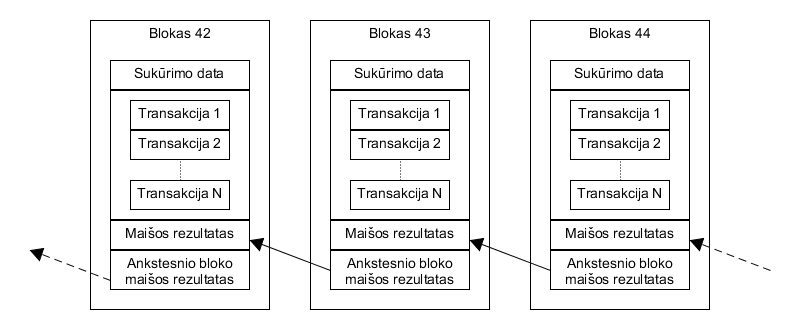
\includegraphics[scale=0.6]{img/blockchain}
    \caption{Supaprastintas blokų grandinės modelis}
    \label{fig:blockchain}
\end{figure}

\subsection{Nekintamumas}

Blokų grandinėje kiekvienas blokas yra sudarytas iš šių dalių:

\begin{itemize}
    \item transakcijų. Kiekviena transakcija yra duomenys, kuriuos norima saugoti blokų grandinėje. Šie duomenys gali būti bet kokia vertinga informacija:
    pervesti pinigai, programinis kodas, skaitmeninės tapatybės atributai ar kt. Kiekviena transakcija yra pasirašoma
    kūrėjo privačiu raktu. Vienas blokas gali turėti vieną arba daugiau transakcijų;
    \item bloko kriptografinės maišos funkcijos rezultato (angl. \textit{hash});
    \item ankstesnio (tėvinio) bloko kriptografinės maišos funkcijos rezultato;
    \item bloko sukūrimo laiko. Blokai grandinėje saugomi chronologiškai;
    \item kitų metaduomenų (pvz. bloko eilės numerio, blokų grandinės versijos, \textit{nonce} darbo įrodymui).
\end{itemize}

Kiekvieno bloko maišos funkcijos rezultatas priklauso nuo jo transakcijų, prieš tai buvusio bloko maišos rezultato ir bloko metaduomenų.
Jeigu betkurio bloko duomenys būtų pakeisti, tuomet maišos funkcija sugeneruotų kitokį maišos rezultatą ir būtų lengva patikrinti, kad
naujai perskaičiuotas maišos rezultatas nesutampa su bloke esančiu rezultatu. Taip pat, kadangi kiekvienas blokas
priklauso nuo prieš tai buvusio bloko, net ir pakeitus vieną iš pirmųjų blokų, pakeitimas būtų pastebimas pridedant naujus blokus ir būtų galima suprasti,
kad turima blokų grandinės versija yra nevalidi (žr.\hypertarget{fig:blockchainNotIntact}{~\ref{fig:blockchainNotIntact}} pav.). Tokiu būdu kiekvienas blokų grandinės blokas patvirtina prieš tai
buvusio bloko integralumą, taip pasiekiant blokų grandinės nekintamumą (angl. \textit{immutability}),
nes perrašyti įrašus blokuose nepastebėtam labai sunku \cite{SatoshiNakamoto}.

\begin{figure}[H]
    \centering
    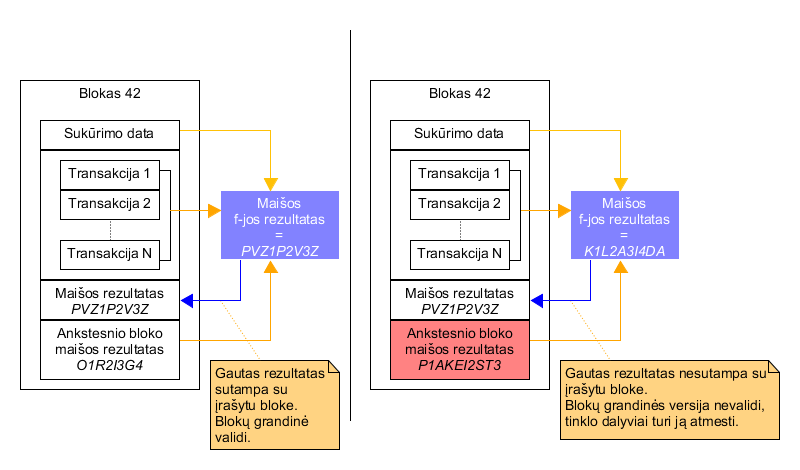
\includegraphics[scale=0.6]{img/blokchainNotIntact}
    \caption{Bloko grandinėje validavimas}
    \label{fig:blockchainNotIntact}
\end{figure}

\subsection{Decentralizuotumas}

Blokų grandinės sistema yra decentralizuota - nėra vieno centrinio serverio, kuris vienas turėtų visą blokų grandinę.
Sistemą sudaro daugybė blokų grandinės mazgų (angl. \textit{node}), kurie turi visą blokų grandinės kopiją. Šie mazgai
yra atsakingi už naujų transakcijų validavimą, blokų su transakcijomis kūrimą, sukurtų blokų priėmimą į blokų grandinę ir pranešimus kitiems mazgams apie naują į grandinę priimtą
bloką \cite{Antonopoulos2016}. Kiekvienas mazgas yra susietas su keletu kitu mazgų. Mazgas, kuris nori pridėti naują bloką (vadinamas \textit{kasėju}), praneša apie jį
kitiems mazgams, jie savo ruožtu žinią perduoda kitiems mazgams ir taip ilgainiui kiekvienas mazgas tinkle turi naujausią blokų grandinės versiją.

Kadangi nėra centrinės institucijos, kuri nuspręstų, ar siūlomas blokas yra tinkamas priimti į grandinę, sprendimą bendrai turi priimti
visi tinklo dalyviai. Egzistuoja skirtingos taisyklės, vadinamos konsensuso strategijomis (plačiau apie juos\hypertarget{blockchain:consensus}{~\ref{blockchain:consensus}} skyrelyje), kuriomis
remdamiesi tinklo mazgai nusprendžia, ar pasiūlytas blokas yra validus. Šios taisyklės apibrėžia, kaip tinklo dalyviai turi įrodyti bloko validumą jį siūlydami į grandinę
bei kaip patikrinti kito dalyvio pasiūlyto bloko validumą.

\subsection{Tipai}

Priklausomai nuo tinklo dalyviams suteikiamų blokų grandinės skaitymo ir rašymo teisių,
išskiriami trys pagrindiniai blokų grandinės tipai: vieša, konsorciumo bei privati.  Tipų skirtumai pateikiami\hypertarget{tab:blockchainComparison}{~\ref{tab:blockchainComparison}} lentelėje.

% \caption{Viešos, konsorciumo ir privačios blokų grandinės palyginimas \cite{Zheng2017}}
% \label{tab:blockchainComparison}
% Table generated by Excel2LaTeX from sheet 'BlockchainComparison'
\begin{table}[htbp]
    \centering
    \caption{Viešos, konsorciumo ir privačios blokų grandinės palyginimas \cite{Zheng2017}}
      \begin{tabular}{|p{8.11em}|l|p{10.22em}|p{6.055em}|}
      \hline
      \multicolumn{1}{|r|}{} & \textbf{Vieša} & \textbf{Konsorciumo} & \textbf{Privati} \bigstrut\\
      \hline
      \textbf{Konsensuso nustatymas} & Visi kasėjai & Išrinkti tinklo dalyviai & Viena organizacija \bigstrut\\
      \hline
      \textbf{Skaitymo teisės} & Viešos & Gali būti viešos ar apribotos & Gali būti viešos ar apribotos \bigstrut\\
      \hline
      \textbf{Centralizuotumas} & Nėra & Dalinis & Yra \bigstrut\\
      \hline
      \textbf{Efektyvumas} & Mažas & Didelis & Didelis \bigstrut\\
      \hline
      \end{tabular}%
    \label{tab:blockchainComparison}%
  \end{table}%
  

Kadangi vieša blokų grandinė yra atvira visam pasauliui, visiems matomos ir joje išsaugotos transakcijos. Tai sudaro puikias salygas įrašų
auditui, tačiau sumažina naudotojų privatumą. Siekiant išlaikyti tam tikrą privatumo lygį, viešoje grandinėje matomi tik transakcijas atlikusių 
asmenų vieši raktai \cite{SatoshiNakamoto}. Viešų blokų grandinių pavyzdžiai: \enquote{Bitcoin}, \enquote{Ethereum} kriptovaliutų blokų grandinės.

Privačios bei konsorciumo blokų grandinės yra tik dalinai decentralizuotos - jose blokų validavimą ir priėmimą į grandinę atlieka vienas
ar dalis tinklo dalyvių. Šios grandinės privalumai: visi validuotojai yra žinomi, grandinės efektyvesnės dėl greičiau priimamų blokų, apribotos blokų skaitymo teisės suteikia didesnį
privatumo lygį, o iškilus poreikiui, tinklo dalyviai gali pakeisti ar atšaukti įvykusias transakcijas \cite{Buterin2015}. Konsorciumo ir privačios blokų grandinės labiau tinkamos įmonių vidiniam (ar jungtiniam,
pvz. tarp kelių finansinių institucijų) naudojimui. Blokų grandinių karkasų sprendimus įmonėms siūlo \enquote{IBM}, \enquote{Microsoft}, \enquote{Amazon} \cite{Zheng2017}.

\subsection{Konsensuso strategijos} \label{blockchain:consensus}

Kadangi blokų grandinės sistema yra decentralizuota, nėra centrinės institucijos, kuri nuspręstų, ar naujai siūlomas pridėti į grandinę blokas
yra validus (be transakcijų su falsifikuotais duomenimis). Todėl blokų grandinės tinkle taikoma konsensuso strategija,
pagal kurią nusprendžiama, ar pridėti naują bloką į grandinę. Apžvelgiamos trys dažnai naudojamos strategijos: darbo, įtakos bei autoriteto įrodymo.

\subsubsection{Darbo įrodymo strategija}

Darbo įrodymo konsensuso strategija remiasi principu, kad daug pastangų ir resursų į bloko validumo įrodymą įdėjęs tinklo
dalyvis nebus linkęs sukčiauti. Šioje strategijoje tinklo dalyvis, norėdamas pridėti bloką į blokų grandinę, turi išspręsti laikui ir resursams
imlų matematinį
uždavinį (užsiima \textit{bloko kasimu}). Pirmas uždavinio reikšmę radęs tinklo dalyvis praneša apie ją kitiems, kurie turi patvirtinti,
ar ši reikšmė teisinga. Jei tai patvirtinta, tinklo dalyviai patikrina, ar naujojo bloko transakcijos yra validžios. Jeigu jos validžios,
blokas pridedamas į grandinę \cite{Zheng2017}.

Darbo įrodymo matematinis uždavinys dažniausiai būna paremtas kriptografine maišos funkcija, kurios rezultatą lengvą validuoti,
tačiau duomenis, sugeneravusius šį rezultatą, sunku surasti. Uždavinio tikslas - surasti šiuos duomenis. Tinklo dalyviai eikvoja didžiulius
kiekius elektros energijos ir laiko,
nes radimas būna paremtas duomenų perrinkimu (angl. \textit{brute force}). Dėl šios priežasties rezultato ieškantiems \textit{kasėjams}
 neretai būna įvesta paskatinimo sistema, kuri teisingą reikšmę radusį
\textit{kasėją} apdovanoja piniginiu atlygiu \cite{SatoshiNakamoto}. 

Kadangi blokų grandinės tinklas yra decentralizuotas, įmanoma situacija, kad labai panašiu metu į grandinę skirtingų mazgų pridėti du validūs blokai.
Taip dalis tinklo dalyvių gaus vieną mazgą, o dalis - kitą, o abu jie bus susieti su tuo pačiu prieš tai buvusiu bloku.
Tokiu atveju, taikoma ilgiausios grandinės taisyklė. Mazgai dirba prie pirmiau gauto bloko,
tačiau išsaugo kitą gautą bloką kaip šaką. Po to, kai bus gautas dar vienas blokas, jis bus susietas tik su viena iš šakų - taip ši šaka taps ilgesnė. Tuomet
ilgesnė šaka paskelbiama aktyviąja grandine, visi su trumpesniąja šaka dirbę mazgai turi pereiti prie aktyviosios grandinės, o atmesto bloko (vadinamo \textit{bloku-našlaičiu}) transakcijos
grąžinamos į bendrą transakcijų sankaupą (angl. \textit{transaction pool}) \cite{SatoshiNakamoto}.
Realiuose blokų grandinės taikymuose, dažnai laukiama keleto iš eilės einančių naujų blokų, kol \textit{blokas-našlaitis}
yra atmetamas. Pavyzdžiui,
\enquote{Bitcoin} blokų grandinėje tik sulaukus apytiksliai 6 blokų iš eilės \textit{blokas-našlaitis} gali būti atmestas\cite{Zheng2017}.

Pagrindinis šios konsensuso strategijos privalumas yra tas, kad dideli kasimo kaštai gali atgrasyti programišius nuo potencialių atakų. Tačiau,
taip veltui išeikvojama daugybė elektros energijos - skaičiuojama, kad kasimas \enquote{Bitcoin} ir \enquote{Ethereum} blokų grandinėms kartu sudėjus per dieną
sueikvoja elektros energijos, kurios vertė yra apie 1 milijoną dolerių \cite{Ethereum}. Taip pat, dėl ilgo uždavinio sprendimo laiko vieno bloko priėmimas į grandinę
gali užtrukti - Bitcoin blokų grandinėje tai užima apie 10 minučių \cite{Zheng2017}.

\subsubsection{Turto įrodymo strategija}

Turto įrodymo konsensuso strategija remiasi principu, kad daug blokų grandinės turto turintis kasėjas
bus sąžiningas, nes išaiškinus jo nesąžiningumą jis rizikuoja prarasti savo turimą turtą \cite{Baars2016}. Šis algoritmas patiki sprendimą priimti
tiems tinklo dalyviams, kurie įrodo kad turi daugiausia turto (pvz. blokų grandinės kriptovaliutos). Remiantis tik šia savybe, tokia strategija gali pasirodyti kaip ne itin sąžininga,
nes turtingiausias tinklo dalyvis gali būti vienvaldžiu sprendimų priėmėju. Dėl to blokų grandinės tinklai neretai taiko patobulintus šios strategijos
variantus: \enquote{Peercoin} papildomai vertina turto amžių, \enquote{Blackcoin} kitą patvirtintoją paskiria pagal atsitiktinę funkciją, kuri atsižvelgia ir į turimą turtą \cite{Zheng2017}.

Ši strategija leidžia nebeeikvoti didžiulių elektros kiekių, skirtingai nei darbo įrodymo strategija \cite{Ethereum}. Algoritmo efektyvumas
taip pat sutaupo laiko ir blokai būna greičiau patvirtinami ir pridedami į grandinę. Tačiau, dėl praktiškai nulinių bloko \textit{kasimo} sąnaudų,
galimos dažnesnės tinklo atakos \cite{Zheng2017}. 

\subsubsection{Autoriteto įrodymo strategija}

Autoriteto įrodymo strategija remiasi keleto tinklo dalyvių, kuriems suteikta teisė validuoti naujus blokus, priimamais sprendimais. Ši strategija nebėra tinkama visiškai
decentralizuotai blokų grandinei, kurioje būtinas pilnas pasitikėjimo padalinimas \cite{ProofOfAuthority}. Tačiau ši strategija tinkama privačioms
ar konsorciumo blokų grandinėms.

Šis konsensuso mechanizmas remiasi iš anksto išrinktais tinklo dalyviais, kurie bus atsakingi už blokų validavimą. Kiekvieną kartą pridedant naują
bloką į grandinę, vienas iš išrinktų validuotojų patvirtins arba atmes pasiūlytą bloką. Siekiant sumažinti galimą kenksmingų patvirtintojų žalą,
įvedamos taisyklės, neleidžiančios tam pačiam validuotojui patvirtinti keleto blokų iš eilės \cite{ProofOfAuthority}.

Autoriteto įrodymo strategijoje validuotojams svarbu išlaikyti gerą reputaciją - susigadinus ją, validuotojas gali būti pašalintas iš tinklo. Šis konsensuso mechanizmas
leidžia greitai ir su itin mažais ištekliais pridėti blokus, tačiau nėra tinkamas pilnai decentralizuotoms blokų grandinėms. Šią strategiją
taiko \enquote{Parity} blokų grandinė \cite{ProofOfAuthority}.

\subsection{Išmanieji kontraktai}

Išmanusis kontraktas (angl. \textit{smart contract}) - tai kompiuterizuotas transakcijos protokolas, kuris
išpildo kontrakto sąlygas, jei patenkinami numatyti kriterij \cite{Szabo1997}.
Išmanųjį kontraktą galima apibūdinti kaip tam tikras sąlygas (išreikštas kodu), kurios, patenkinus reikalavimus, bus įvykdytos automatiškai,
be trečiosios šalies priežiūros.

Idėja, pristatyta dar prieš 2000-uosius, šiais laikais yra įgyvendinama pasitelkiant blokų grandinę. Išmanusis kontraktas
į blokų grandinę yra patalpinamas kaip transakcija. Tuomet, dėl blokų grandinės viešumo, kodo logika būna atskleista ir kiekvienas norintis
gali įsitikinti, ar kontraktas veiks tinkamai. Taip pat, kadangi pats išmanusis kontraktas yra blokų grandinės transakcijoje, jis nebegali būti keičiamas.
Tai padidina naudotojų pasitikėjimą, nes jokia centrinė institucija negali
pakeisti kontrakto sąlygų. Tačiau, jei kode palikta defektų, jų nebebus galima ištaisyti.

Blokų grandinėje esančių išmaniųjų kontraktų kodas yra vykdomas automatiškai tinkle esančių kasėjų \cite{Zheng2017}.
Taip nebelieka vienintelio nesekmės taško situacijos, kai kodą vykdytų vienas centrinis serveris - išmaniojo kontrakto
kodas butų nebevykdomas tik tada, jei visi tinklo mazgai išeitų iš tinklo. Už tai, kad tinklo dalyviai naudoja savo kompiuterių
resursus išmaniųjų kontraktų kodui vykdyti, jiems dažniausiai suteikiamas piniginis paskatinimas.

Išmaniųjų kontraktų veikimo detalės priklauso nuo blokų grandinės, kurioje jie bus vykdomi.
Bene žinomiausia išmaniųjų kontraktų kūrimui pritaikyta platforma - \enquote{Ethereum}.
\hypertarget{section:ethereumIntro}{\ref{section:ethereumIntro}} skyrelyje apžvelgiamos pagrindinės išmaniųjų kontraktų
veikimo sąlygos.

\subsubsection{\enquote{Ethereum} išmanieji kontraktai} \label{section:ethereumIntro}

2015-aisias pradėjusi veikti \enquote{Ethereum} platforma pristatė blokų grandinę, kuri pritaikyta kurti būseną galinčius keisti
išmaniuosius kontraktus su išbaigta
(angl. \textit{turing complete}) programavimo kalba \cite{EthereumWhitePaper}. \enquote{Ethereum} kontraktai vykdomi tinklo
dalyvių, \enquote{Ethereum} virtualiosios mašinos pagalba.  \enquote{Ethereum} virtualioji mašina gali būti suprantama kaip didelis decentralizuotas
kompiuteris, saugantis milijonus objektų, vadinamų paskyromis, kurie turi galimybę turėti savo duomenis,
vykdyti kodą bei bendrauti tarpusavyje \cite{Ethereum}.

\enquote{Ethereum} platforma turi paskyras, kuriomis naudojantis, galima kurti transakcijas bei kviesti išmaniųjų
kontraktų funkcijas. Paskyros identifikuojamos pagal unikalų adresą. \enquote{Ethereum} egzistuoja dviejų tipų paskyros \cite{Ethereum}:

\begin{enumerate}
    \item išorinės paskyros (angl. \textit{externally owned accounts}). Jos savininkų valdomos privačiais raktais ir turi eterio
    balansą;
    \item kontraktų paskyros (angl. \textit{contract accounts}). Šios paskyros be balanso turi kodą bei būseną, kuri gali keistis,
    jei įvykdomos kode aprašytos sąlygos. Kontraktų paskyros yra valdomos kontrakto kodo.
\end{enumerate}

Skatinant tinklo dalyvius vykdyti kontraktų kodą, jiems už šį darbą skiriama piniginė premija - eterio kriptovaliuta. Kiek eterio
bus skiriama, priklauso nuo vykdomo kodo sudėtingumo ir jam reikalingų resursų. Dėl to kiekviena kodo operacija \enquote{Ethereum} platformoje
yra įvertinama kuro (angl. \textit{gas}) kiekiu, kuris nurodo sąlyginę kainą. Kuro sistema padeda apsisaugoti nuo begalinių ciklų vykdymų - jei vykdant
funkciją baigiasi kuras, vykdymas nutraukiamas, o kuras kvietėjui nėra grąžinamas \cite{EthereumWhitePaper}.\\
Skiriamos dviejų tipų funkcijos: rašymo bei skaitymo. Skaitymo funkcijų kvietimas yra nemokamas - jos tik grąžina
esamus kontrakto duomenis. Rašymo funkcijos yra mokamos, nes jos keičia kontrakto būseną. Jų vykdymo metu turi būti sukurta transakcija,
kurią patvirtins \enquote{Ethereum} blokų grandinės dalyviai. Kuo didesnis duomenų kiekis bus išsaugotas būsenoje, tuo brangesnė bus operacija.

Funkcijos kvietimą apmoka kvietėjas. Dėl šios priežasties kvietėjas savo paskyroje turi turėti eterio, iš kurio galės padengti
kviečiamos funkcijos išlaidas. Norint neversti kvietėjo apmokėti, kontrakto kodas kviečiamos funkcijos pabaigoje gali į kvietėjo paskyrą
pervesti jo išeikvotą eterį. Tolimesnėse \enquote{Ethereum} versijose svarstoma įdiegti funkcionalumą,
kuris standartizuotų būdą, leisiantį kontraktams patiems apmokėti iškviestų funkcijų išlaidas \cite{ContractPays}.

Bendravimui su vartotojui skirtomis klientinėmis programomis, komunikuojančiomis su blokų grandine (neretai vadinamoms \textit{dapp}), \enquote{Ethereum} platformoje dažniausiai naudojami
įvykiai (angl. \textit{events}). Išmaniajame kontrakte galima apibrėžti įvykį ir jo grąžinamus duomenis. Į kontrakto funkcijas tuomet
pridedamas kodas, kuris paskelbs įvykį su pasirinktais duomenimis. Visos klientinės programos,
besiklausančios šio įvykio, bus informuotos ir gaus įvykyje perduotus duomenis. Taip klientinė programa gali reaguoti į išmaniajame
kontrakte įvykusius pokyčius.\\
Įvykiai \enquote{Ethereum} blokų grandinėje saugomi kaip registrai (angl. \textit{logs}), o paskelbti įvykius kainuoja gerokai mažiau kuro,
nei keisti kontrakto būseną. Dėl šios priežasties įvykius galima naudoti kaip pigesnę alternatyvą duomenims blokų grandinėje saugoti. Tačiau, įvykiuose paskelbti
duomenys nėra prieinami iš išmaniojo kontrakto kodo \cite{EthereumWhitePaper}.

\subsection{Pavojai ir trūkumai} \label{blockchain:concerns}

Blokų grandinės technologija sukuria sąlygas decentralizuotai, nesuteikiant pasitikėjimo vienam ar keliems dalyviams, laikyti nekeičiamus duomenis.
Tai atveria įvairių galimybių finansų, daiktų interneto, reputacijos sistemų ar saugumo srityse \cite{Zheng2017}, tačiau ši technologija turi ir trūkumų,
kurių galimą poveikį būtina įvertinti prieš taikant šią technologiją konkrečioje sferoje. Pagrindinės grėsmės ir trūkumai aptariami šiame skyriuje.

\subsubsection{Daugumos ataka}

Viešose blokų grandinėse dauguma (>50\%) mazgų tinkle turi patvirtinti bloką, kad jis būtų priimtas į grandinę. Potencialus įsilaužėlis gali pateikti
falsifikuotą blokų grandinės bloką (pvz. su netikromis transakcijomis), tačiau kol jis neturi daugumos skaičiavimo galios tinkle, šis blokas bus
atmestas likusių dalyvių mazge (ir taps \textit{bloku-našlaičiu} taikant ilgiausios grandinės taisyklę). Tačiau, jeigu įsilaužėlis (ar keletas jų)
turi daugumą skaičiavimo galios, jis gali dirbti su falsifikuota blokų grandinės versija greičiau negu likę dalyviai tinkle ir taip ilgiausia grandine, prie kurios
pereis visi dalyviai, taps jo sukurta grandinė su falsifikuotais blokais \cite{Zheng2017}. Ši ataka nebuvo įgyvendinta prieš žinomiausias \enquote{Bitcoin} bei \enquote{Ethereum} blokų grandines, tačiau
buvo įvykdyta prieš \enquote{Verge} blokų grandinę \cite{Sedgwick2018}.

\subsubsection{Plečiamumas}

Blokų grandinės plečiamumas matuojamas pagal du kriterijus: transakcijų pralaidumą ir saugojimo reikalavimus mazgams. Transakcijų pralaidumas, kuris priklauso nuo to,
kaip greitai nauji blokai yra pridedami į blokų grandinę, susijęs su taikoma konsensuso strategija.
Kuo taikoma strategija leidžia greičiau priimti naują bloką, tuo greičiau transakcijos bus patvirtintos. \enquote{Bitcoin} kriptovaliutos blokų grandinėje, taikančioje darbo įrodymo konsensusą,
apdorojoma apie 7 transakcijas per sekundę \cite{Zheng2017}, kai \enquote{Tendermint} blokų grandinė, taikanti
atsparumo klaidoms konsensusą, teigia galinti apdoroti tūkstančius transakcijų per sekundę \cite{Tendermint2017}. Dėl darbo įrodymo strategijos neefektyvumo
blokų grandinės neretai tampa priverstos iškeisti ją į efektyvesnį konsensuso būdą - \enquote{Ethereum} blokų grandinė ketina pereiti prie turto įrodymu grįsto konsensuso \cite{Ethereum}.

Kita priežastis, dėl ko transakcijos tvirtinamos gana lėtai - blokai turi dydžio apribojimus. Dėl šių apribojimų, tik dalis susikaupusių transakcijų gali būti priimtos
į naują bloką, o likusios turi laukti, kol pateks į kitą bloką. Tam spręsti pasitelktos šalutinės blokų grandinės. Jos dalį bloko duomenų iškelia į šalutinę grandinę,
taip palikdamos daugiau vietos pagrindinės grandinės bloke. Tokį sprendimą priėmė \enquote{Bitcoin} blokų grandinė, į tinklą pristatydama \enquote{SegWit} protokolą, kuris iškelia skaitmeninių
parašų duomenis į atskirą grandinę \cite{Segwit}.

Visos blokų grandinės dydis taip pat gali sukelti plečiamumo problemų. Šiuo metu Bitcoin blokų grandinė užima per 100 gigabaitų \cite{Zheng2017}. Siekiant sumažinti blokų grandinės
(kurią turi kiekvienas mazgas tinkle) dydį,
siūlomi įvairūs sprendimai. Vienas variantas yra mazgams neturėti seniausių blokų grandinės dalių, o senus blokus su transakcijomis iškelti į atskirą duomenų bazę.
Kitas sprendimo būdas - pagrindinėje blokų grandinėje laikyti tik transakcijų maišos rezultatus, o pačius transakcijų duomenis
iškelti už grandinės ribų (angl. \textit{off-chain}) \cite{Lo2017}.

\subsubsection{Anonimiškumas}

Manoma, kad blokų grandinės išsaugo naudotojų privatumą dėl to, kad transakcijose atskleidžiamas tik naudotojų
viešas raktos vietoj tikrosios tapatybės \cite{Zheng2017}. Tačiau, tyrimai rodo, kad iš viešojo rakto galima
atsekti tikrąją naudotojo tapatybę \cite{Barcelo2007}. Taip pat, transakcijoje buvę duomenys (pvz. pervestas pinigų kiekis)
viešoje blokų grandinėje bus matomas visiems tinklo dalyviams.

Galimi skirtingi sprendimai didesniam anonimiškumui pasiekti. Pirmiausia, reikia atsižvelgti, ar negalima naudoti privačios blokų grandinės, kurioje
blokų skaitymo teisės būtų apribotos. Kitas variantas - blokų grandinėje saugoti užšifruotus duomenis, kurių skaitymui
reikia turėti dešifravimo raktą. Jeigu tai netinkama išeitis, tuomet transakcijas galima atlikti per tarpininką, kuris išskaidys vieną transakciją
į keletą, vykdomų su skirtingais viešaisiais raktais, ir taip bus sunkiau atsekti transakcijos autorių \cite{Zheng2017}.

